
\subsection{Random Access Parser Design Pattern}

\subsubsection{Intent}
The Random Access Parser design pattern creates a navigable data structure from plain and large files that follows certain format, making it easier to access data records in both directions, backward and forward, while operating over them. Navigating the data structure produces per-record snapshots that are written to disk, which reduces reading time and memory consumption.

\subsubsection{Problem}
Usually, processing a large file of structured data (e.g., XML or JSON) requires different kinds of operations, for example, to insert, remove, and update data records in a data base management system. The structured data can follow a standard format, typically some conceptual variation of the WebRowSet format. The WebRowSet format comprises three parts: properties, metadata, and data. In the context of the previous example, the properties section contains details regarding the Relational Database Management System (e.g., synchronization provider, isolation level, and rowset type). The metadata section contains information about the database structure (e.g., column numbers, their names, and types). Finally, the data section contains the application data.

For the processing, data records might be required to be accessed randomly and refer to other records, located possible far before or after the current one. Another example is if a file can be processed per table, this requires to read not only the concrete data but also the associated metadata and properties. In case the metadata or properties are modified, it is likely the data would need to be also modified; performing such modifications imply moving forward and backwards in the file, therefore this can introduce performance issues. These issues are commonly caused because an efficient processing would imply to load the whole file into memory, which is not possible.

\subsubsection{Context}
Typical processing of data sets requires to iterate over the data records. Even though these data sets may be very large, a common approach is to load all the data into main memory. However, this affects negatively the overall application performance, and in some cases, it is not even possible to load the whole file into memory. For this reason, on-demand reading is desired and sometimes, required. Moreover, this strategy allows the processing to behave scalable and stable, in terms of time and memory consumption.

\subsubsection{Forces}
\textbf{\textit{Efficiently random access to a large structured data file.}} This design pattern proposes the use of two lookup tables. On the one hand, one table is used to remember the already read, updated, inserted, or deleted data records through parser snapshots using the memento design pattern. On the other hand, the other table is used to maintain the original data structure. These snapshots allow an efficient and manageable random access and avoid memory overflow caused by the processing of large files.

\subsubsection{Structure Diagram - Figure \ref{fig:str_diagram_rap}}

\begin{figure}
	\centering
	\includegraphics*[width=1\textwidth, keepaspectratio=false]{fig/image1.eps}
	\caption{Structure Diagram - Random Access Parser Design Pattern}
	\label{fig:str_diagram_rap}
\end{figure}

\begin{description}
	\item[Participants]
\end{description}

\begin{description}
	\item[Domain Specific Parser:]
	An abstract class that contains the abstract method \textit{parse}. This method allows to transform the contents of a file into a data structure, for instance, the corresponding data structure for the XML or JSON formats.
	
	\item[Concrete Parser:]
	A concrete implementation of the DomainSpecifParser class. It is responsible for implementing the \textit{parse} method. Some well known implementations of the ConcreteParser class can be found for XML-parsing libraries such as SAX, Dom and XPath.
	
	\item[Lookup Table:]
	This component allows to navigate inside memento snapshots.
	
	\item[Table Element:]
	This component is responsible to encapsulate and identify each memento element.
	
	\item[Memento:]
	Memento is a design pattern designed to save a specific object state. Given that the object states are saved, it can roll back to a previous state.
	
	\item[Random Access Parser:]
	This is the main component. It is responsible for reading a file, transforming it into a data structure by means of a ConcreteParser, performing operations (i.e., update, delete, insert) over the data structure, storing and restoring states of the data structure.
	
\end{description}

\subsubsection{Behavior}

%\begin{figure}
%	\centering
%	\includegraphics*[width=0.8\textwidth, keepaspectratio=false]{fig/image2.eps}
%	\caption{Initialization Sequence Diagram - Random Access Parser Design Pattern}
%	\label{fig:init_seq_diagram_rap}
%\end{figure}

\begin{figure}
	\centering
	\includegraphics*[width=1\textwidth, keepaspectratio=false]{fig/image3.eps}
	\caption{Processing Sequence Diagram - Random Access Parser Design Pattern}
	\label{fig:proc_seq_diagram_rap}
\end{figure}

%\begin{description}
%	\item[Scenarios]
%\end{description}

\begin{description}
	%	\item[Initialization Scenario - Figure \ref{fig:init_seq_diagram_rap}]
	%	This scenario describes how the design pattern is configured initially. To configure initially the design pattern a request to process a file must arrive, when file path is sent to RandomAccessParser, it calls the concrete parser for interpreting the file and the parser returns the corresponding DataStructure.
	
	
	\item[Processing Scenario - Figure \ref{fig:proc_seq_diagram_rap} ].\\
	This scenario describes the normal processing behavior of RandomAccessParser design pattern.
	
	\begin{itemize}
		\item  When any record is requested, no matter its location, RandomAccessParser searches into its LookUpTable the required element.
		
		\item  The LookUpTable searches in its TableElements the right element according to the elementId.
		
		\item  Once the correct TableElement is found, it gets its associated Memento object, and the memento is returned to the RandomAccessParser, which returns the DataStructureRecord.
	\end{itemize}
	
\end{description}

\subsection{Reactor Design Pattern}

\subsubsection{Intent}
The Reactor design pattern handles different types of concurrent service requests that are delivered by one or several clients. Service requests are received by a service-specific event handler, working separately from the service implementation. These event handlers are registered into a dispatcher, which is in charge of executing the corresponding services.


\subsubsection{Context}
A server application concurrently serves several types of service requests from one or more distributed clients. These requests are internally handled as events by event handlers.


\subsubsection{Problem}
In distributed environments, servers offer different services, and a single server can receive different request types. Processing a request can imply locks in the requests arrival point, while client requests are serviced. These locks can impact negatively the system performance.

Additionally, different request types require different handlers, hence it is necessary to select the adequate ones. This selection performed dynamically increases the time to respond each request. A typical solution is to use a thread for each request, however this solution implies system overhead when threads finish processing and become idle, especially when requests are not uniformly distributed among request types.


\subsubsection{Forces}
\textbf{\textit{Favor service availability. }}This pattern uses a dispatcher to redirect requests to the corresponding handlers, therefore the server does not block while attending a single request. \\

\noindent\textbf{\textit{Increase server efficiency.}} By using a request dispatcher, and by avoiding idle threads in request processing this pattern aims at reducing unnecessary use of CPUs and minimizing latency in service requests, and maximizes throughput.\\

\noindent\textbf{\textit{Ease service adaptability.}} Given that handlers are registered with a single request dispatcher, this pattern eases modifying or adding handlers for different types of service requests.

\subsubsection{Structure Diagram - Figure \ref{fig:str_diagram_r}}

\begin{figure}
	\centering
	\includegraphics*[width=1\textwidth, keepaspectratio=false]{fig/image4.eps}
	\caption{Structure Diagram - Reactor Design Pattern}
	\label{fig:str_diagram_r}
\end{figure}


\begin{description}
	\item[Participants]
\end{description}

\begin{description}
	\item[Request Processor:]
	Represents the requests reception point. This class contains the necessary information to redirect the request to the corresponding handler to process the service request.
	
	\item[Request Handler Interface:]
	An interface specifying the required service to handle requests. The service specified by this interface must be implemented by concrete request handlers. 
	
	\item[Concrete Request Handler:]
	A concrete class implementing the request handler interface.  Concrete request handlers are registered with the initiation dispatcher. When a request corresponding to the request handler type arrives, it is called by the initiation dispatcher.
	
	\item[Synchronous Request Demultiplexer:]
	Waits for a request to occur, and returns a handler without blocking the initiation dispatcher. Thus allowing the system to continue serving requests.
	
	\item[Initiation Dispatcher:]
	Responsible for both registering and removing request handlers, and dispatching service requests. It waits for requests to be processed by the synchronous request demultiplexer component, and calls the concrete request handler component to process each request.
\end{description}

\subsubsection{Behavior}

%\begin{figure}
%	\centering
%	\includegraphics*[width=0.8\textwidth, keepaspectratio=false]{fig/image5.eps}
%	\caption{Sequence Diagram Initialization - Reactor Design Pattern}
%	\label{fig:seq_diagram_r}
%\end{figure}

\begin{figure}[ht!]
	\centering
	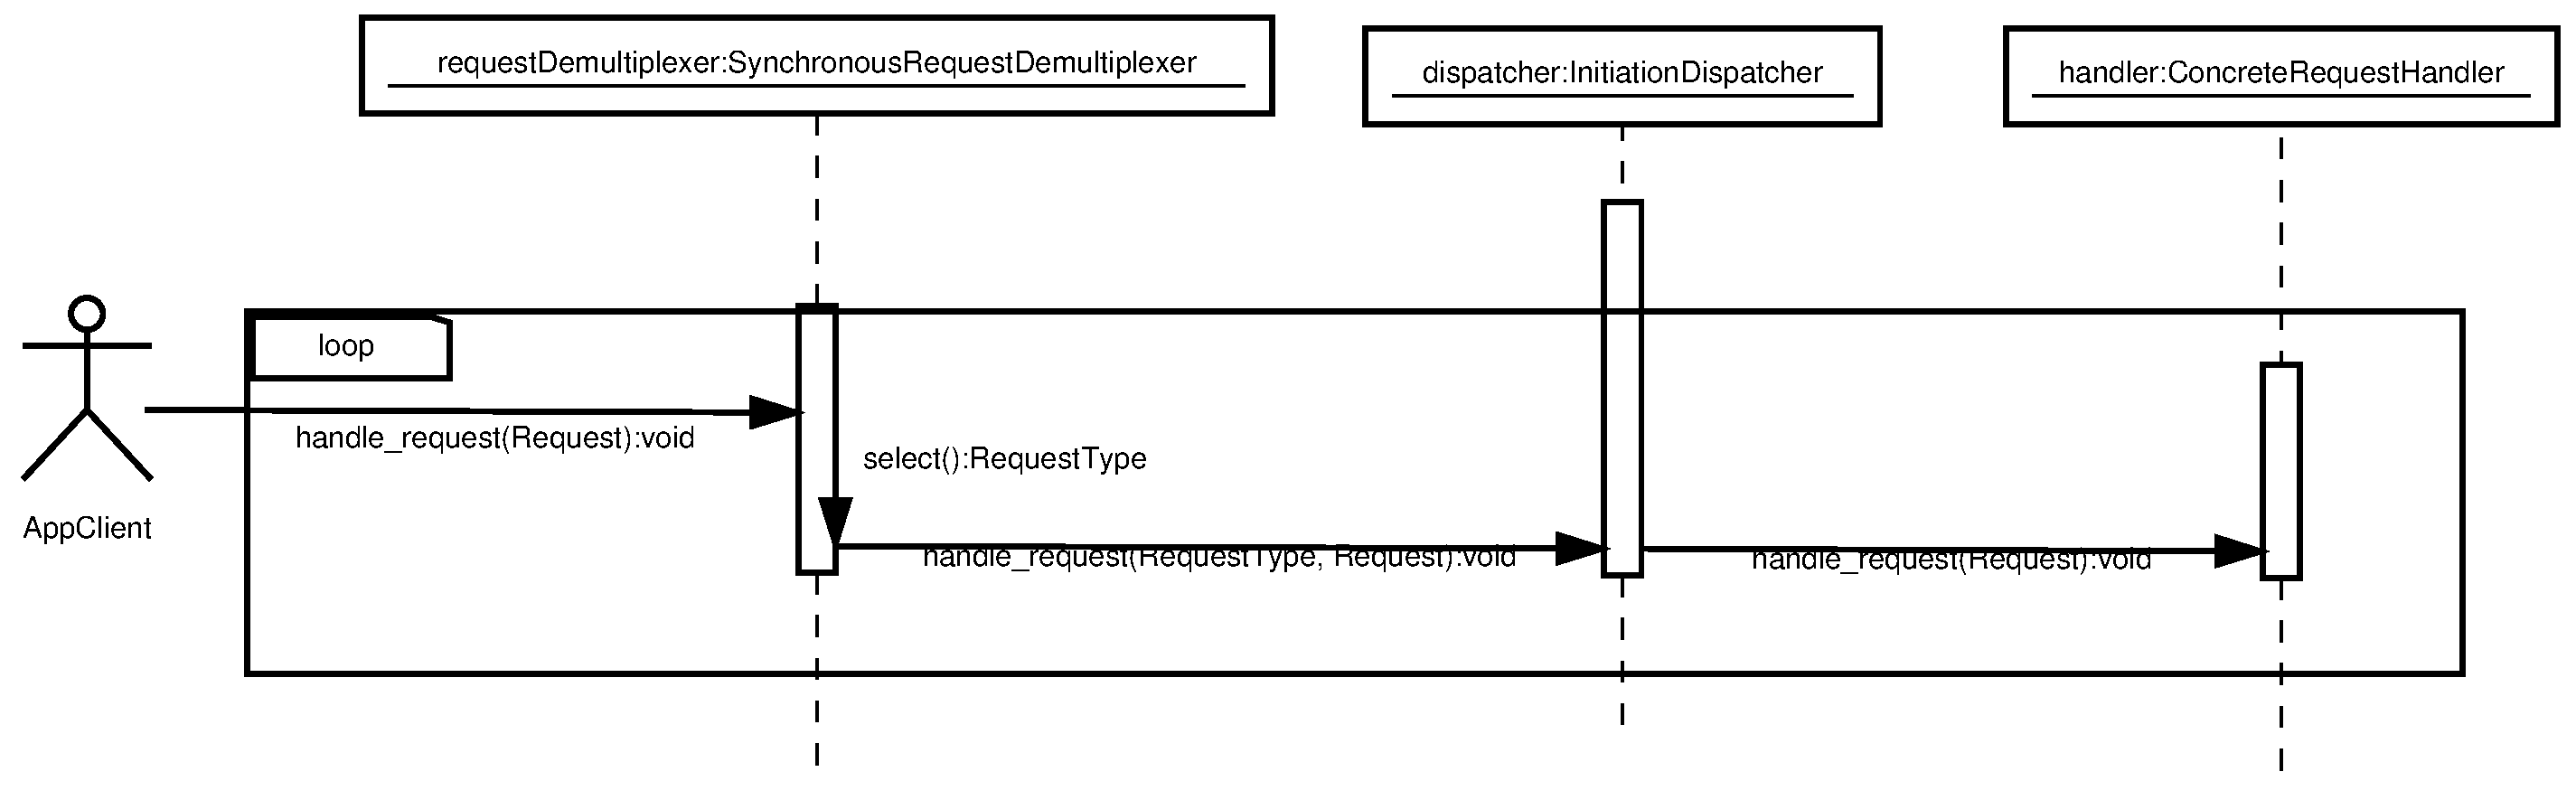
\includegraphics[width=1\textwidth]{fig/image32.eps}
	\caption{Request Processing Sequence Diagram - Reactor}
	\label{fig:seq_diagram_r2}
\end{figure}


%\begin{description}
%	\item[Scenarios]
%\end{description}

%\begin{description}
%	\item[Figure \ref{fig:seq_diagram_r} - Reactor Design Pattern]
%\end{description}

\begin{description}
	\item[Processing Scenario - Figure \ref{fig:seq_diagram_r2}].\\
	
	\begin{itemize}
		\item  When an Event handler is registered in the Initiation dispatcher, a type of event is specified by the application registering the handler; when an event of this type occur on the associated Handle, the Event handler will be notified.
		
		\item  The Initiation dispatcher gets the associated Handle from Event handlers once they are registered.
		
		\item  After all the Event handlers are registered, the event loop is started in the Initiation dispatcher by an application. So, the Synchronous event demultiplexer is executed and it is put on wait for events.
		
		\item  When a new event arrives (i.e., a Handle becomes ``ready''), the Synchronous event demultiplexer notifies the Initiation dispatcher.
		
		\item  When the Initiation dispatcher is notified about a new event, it calls the corresponding Event handler callback method. The initiation dispatcher uses the Handles to find the appropriate Event handler callback method.
		
		\item  The Initiation Dispatcher calls back to the handle event hook method of the Event Handler to perform application-specific functionality in response to an event.
	\end{itemize}
\end{description}

\subsection{State-based Pipeline Design Pattern}

\subsubsection{Intent}
The State-based Pipeline design pattern takes advantage of the simplicity of the Pipeline design pattern, and the efficient execution of a master/slave structure. This variant of the original pipeline design pattern reduces prominent downsides for coarse--grained applications in achieving good performance, namely: first, when the pipeline is not full (i.e., at the beginning and end of the pipeline) stages are idle; second, load balancing is crucial to achieve good performance, as expensive stages cause that less expensive stages stay idle; and third, it is difficult to incrementally add more processors into an existing pipeline, given that concurrency in a pipeline is tightly coupled with the set of stages.

\subsubsection{Problem}
The pipeline structure has demonstrated to be a useful way to solve many practical problems in parallel computing programming; however, it presents three serious problems, especially for coarse-grained applications. 

\begin{itemize}
	\item  Processors are idle when the pipeline is at the beginning and the end of the process.
	      
	\item  Traditional pipeline implementations are sensitive to load imbalance, this means that some pipelines stages are more time-consuming than others. The slowest stage will become a bottleneck, decreasing the performance.
	      
	\item  Traditional pipeline implementations imply static assignment of the stages to the nodes, making difficult to take advantage of new nodes.
\end{itemize}

\subsubsection{Context}
A pipeline consists of a set of ordered stages, where each stage receives data from its predecessor, transforms that data, and finally sends it to the next stage. Usually, for data transference it is necessary to place buffers between the stages.

The paramount characteristic in pipeline is that each stage is independent. That is, each stage can perform different computations on different parts of the data, simultaneously.

However, Pipeline presents serious performance problems as ramp-up and ramp-down time, and load imbalance. 

The state-based pipeline should be used when:

\begin{itemize}
	\item  Load balance must be guaranteed.
	      
	\item  New processor or stages could be available at any time and should be taken advantage of.
\end{itemize}

\subsubsection{Forces}
\textbf{\textit{Decouple the concurrency from the pipeline structure}}. By using the State-based Pipeline design pattern, stages (i.e., state transitions) are independent of the execution thread, improving load balancing between pipeline stages and reducing idle times.\\

\noindent\textbf{\textit{Clarify transitions between stages}}. There should be a clear agreement on the order in which the transformations occur from one stage to another. Thus if it is required, this makes it simple to add, modify or reorder states in the pipeline.

\subsubsection{Structure Diagram - Figure \ref{fig:str_diagram_sbp}} 

\begin{figure}
	\centering
	\includegraphics*[width=0.9\textwidth, keepaspectratio=false]{fig/image6.eps}
	\caption{Structure Diagram - State-based Pipeline Design Pattern}
	\label{fig:str_diagram_sbp}
\end{figure}


\begin{description}
	\item[Participants]
\end{description}

\begin{description}
	\item[AbstractStage]
	An abstract representation of the stages, containing an abstract method to transform one stage into another.
	
	\item[ConcreteStage]
	Represents a stage within the pipeline. Its method returns a concrete stage (the subsequent stage).
	
	\item[Pipeline]
	This class contains the configured concrete stages, the queues storing intermediate states (i.e., instances of ConcreteStage), and the slave threads consuming objects from the queues.
	
\end{description}

\subsubsection{Behavior}

\begin{figure}
	\centering
	\includegraphics*[width=1\textwidth,, keepaspectratio=false]{fig/StateBehavior.eps}
	\caption{Processing Sequence Diagram - State-based Pipeline Design Pattern}
	\label{fig:seq_diagram_sbp}
\end{figure}

%\begin{description}
%	\item[Scenarios]
%\end{description}

\begin{description}
	\item[Processing Scenario - Figure \ref{fig:seq_diagram_sbp}]
\end{description}

\begin{itemize}
	\item  Put the request objects into the input buffer.
	      
	\item  An idle thread from the thread pool will find and execute the transform() method of any object request from any buffer placed between stages, in order to obtain the next state object.
	      
	\item  The state object resulting from transform () method is placed into an output buffer proper of its runtime type.
	      
	\item  The final buffer holds the resulting output objects from the pipeline execution.
\end{itemize}

\subsection{Thread Pool Design Pattern}
\label{subsec:threadpool}

\subsubsection{Intent}
The thread pool design pattern facilitates thread management. In parallel environments, where some tasks can be executed at same time but perhaps in different instantiations, in the same device, threads should be used. Each thread executes an own task and shares device resources. When many threads are executed in the same device concurrently, resources could not be enough and overrun device capacity. 

\subsubsection{Problem}
Concurrency is usually realized having several threads executed in a computing device. However, each of these threads consume device resources, and eventually, many threads might overload the device. Managing these threads represents a problem. For example, Can threads be reused? What would be the maximum or minimum amount of threads for device?

\subsubsection{Context}
In general, each time a problem solution requires using concurrent execution of threads, this pattern can be used. Threads are used to execute several independent computing tasks at the same time, however these threads imply costs in time (i.e., time to start a thread) and resources (memory and CPU). This pattern proposes a solution that balances the implications of using threads. Furthermore, many other patterns that imply the use of threads implement this pattern as part of their solution. This is the case for instance with the leader/followers and master/workers design patterns.Despite of this pattern allows to take advantage of the multi-core environment of a CPU and this can improve the system performance, it has limitations, such as, difficult to scale the pattern implementation to a distributed environment (i.e., applying this pattern using many processing nodes).

\subsubsection{Forces}
\textbf{\textit{All tasks should be independent}}. Each of the tasks should be executable fully and independently in one thread. If there are dependencies, deadlocks can happen. For instance, if all pool's threads is waiting for other task, this task will not be executed and thus threads could enter in deadlocks.\\

\noindent\textbf{\textit{Thread creation cost is relatively high}}. To create a thread for each task should be costlier than maintaining and waiting for idle threads, both in terms of time and resources.\\

\noindent\textbf{\textit{Optimal threads amount}}. Designer should configure the optimal threads amount depending on the device resource availability and execution capability at the same time. This relation should be maintained dynamically, as the device load evolves.\\

\noindent\textbf{\textit{Threads not reusable.}} If a task lasts indefinitely, the thread that executes this task is not reusable because it may never terminate to execute the task. This task type should be executed by a thread out of pool.

\subsubsection{Structure Diagram - Figure \ref{fig:str_diagram_tp}}

\begin{figure}
	\centering
	\includegraphics*[width=0.7\textwidth, keepaspectratio=false]{fig/image8.eps}
	\caption{Structure Diagram - Thread Pool Design Pattern}
	\label{fig:str_diagram_tp}
\end{figure}

\begin{description}
	\item[Participants]
\end{description}

\begin{description}
	\item[Worker:]
	Responsible to execute tasks of ThreadPool. This gets Runnable objects from its ThreadPool, by executing the Runnable method.
	
	\item[Runnable:]
	Represents the interface implemented by tasks that ThreadPool must process. This interface specifies the \textbf{\textit{run }}method, which is responsible for defining the task of the Runnable object.
	
	\item[ThreadPool:]
	ThreadPool class is responsible for managing workers and tasks and their execution. This class assigns to each worker one task. When a worker finishes a task execution, it can ask the threadpool for a new task. 
	
	\item[Executor:]
	Represents the interface implemented by ThreadPool class. This interface specifies the \textbf{\textit{execute }}method, which is responsible for executing the task of the Runnable object.
	
\end{description}

\subsubsection{Behavior}

%\begin{figure}
%	\centering
%	\includegraphics*[width=1\textwidth, keepaspectratio=false]{fig/image9.eps}
%	\caption{Sequence Diagram Initialization Scenario - Thread Pool Design Pattern}
%	\label{fig:seq_diagram_tp1}
%\end{figure}

\begin{figure}
	\centering
	\includegraphics*[width=1\textwidth, keepaspectratio=false]{fig/image30.eps}
	\caption{Request Processing Sequence Diagram - Thread Pool}
	\label{fig:seq_diagram_tp2}
\end{figure}


%\begin{description}
%	\item[Scenarios]
%\end{description}

\begin{description}
	%	\item[Initialization - Figure \ref{fig:seq_diagram_tp1}]
	%	The initial configuration of this pattern depends on requests to execute tasks, every time a request arrives it is verified if idle threads exists, otherwise, if the maximum thread amount is not exceed, a new thread is created.
	
	\item[Processing Scenario - Figure \ref{fig:seq_diagram_tp2}].\\
	Every time a request arrives it is verified if idle threads exists, otherwise, if the maximum thread amount is not exceed, a new thread is created. If exists at least one thread available to process a request, the pool sends the request to be executed, otherwise the request must wait until a thread become idle. Finally, the thread returns to the pool as idle thread when processing of the request is finished.
\end{description}


\subsection{Master-Worker Design Pattern}
\label{sebsec:mw_design_pattern}
Also known as:

\begin{itemize}
	\item  The Embarrassingly Parallel Pattern
	\item  Task Queue
	\item  Master-Slave
\end{itemize}

\subsubsection{Intent}
The Master-Worker design pattern describes how to execute a collection of independent tasks (i.e., tasks than can be executed concurrently) in a group of available processors, named workers. Furthermore, the distribution of tasks among processors can be performed statically or dynamically in order to promote a balanced computational load.

\subsubsection{Problem}
Many computational problems are solved by splitting them in independent subproblems, such that their solution implementations can be executed independently and concurrently. The independence among subproblems imply that tasks associated to each solution implementation do not share read and write data and tasks must not wait for other task results. Practitioners should take advantage of available computational resources and the inherent concurrency without incurring in unnecessary overhead. Given this situation, a program should be designed procuring to load balance among available processing units.

To exemplify this type of problems, take the vector-addition problem. Given vectors A, B, and C where C=A+B, each element of C is given by adding the corresponding elements of A and B, Ci= Ai + Bi. Each element of C can be calculated in a concurrent way as a set of subproblems of vector elements addition problem.

\subsubsection{Context}
Problems whose solutions can be split in independent tasks can take advantage of this design pattern. However, some particularities should be evaluated before to implement it, (i) cost to initialize workers (including e.g., data transmission) must be lower than the task cost, (ii) number of tasks must be greater than available processing units, and (iii) distribution should be dynamic if load for each task is unknown, or varies unpredictably or when the available load supported by each worker is unknown.

\subsubsection{Forces}
\textbf{\textit{Task must be independent.  }}The Master-Worker design pattern applies when tasks do not have dependencies among them. Otherwise, the tasks must be redesigned to eliminate these dependencies.\\

\noindent\textbf{\textit{Tradeoffs between data communication and load. }}To apply this design pattern the task size must be optimal according to tradeoffs between distribution overhead and task implied load. Given that the size of tasks in Master-Worker can vary from one task to another. \\

\noindent\textbf{\textit{Unpredictable tasks number and processor nodes. }}Most of the time explicit predictions of the hardware and software runtime environment are not possible. However, Master-Worker procures to achieve load balancing even under uncertain environments, by allocating tasks to idle processor nodes. This scenario corresponds to the dynamic version of Master-Worker and also to the Fork-Join design pattern.\\

\noindent\textbf{\textit{Number of tasks and processor nodes are known. }}When the number of tasks and load of processor nodes is known prior to execution, practitioners can program the software to assign statically tasks to the most suitable processor node guaranteeing load balancing. This scenario corresponds to the static version of Master-Worker\footnote{ Some authors do not consider the behavior described by the static version of the Master-Worker design pattern as part of this design pattern, instead they prefer to describe this behavior as a whole new design pattern.}.

\subsubsection{Structure Diagram - Figure \ref{fig:str_diagram_mw}}

\begin{figure}
	\centering
	\includegraphics*[width=0.8\textwidth, keepaspectratio=false]{fig/image7.eps}
	\caption{Structure Diagram - Master-Worker Design Pattern}
	\label{fig:str_diagram_mw}
\end{figure}


\begin{description}
	\item[Participants]
\end{description}

\begin{description}
	\item[Master]
	\label{it:masterdesc}
	The Master contains the shared collection of tasks, usually a queue, where tasks are stored after being split.  It has a second shared queue where results of worker computations are stored. In summary, the Master holds registered tasks, launches the processors (workers) and collects the workers' results to produce the final result.
	
	\item[Worker]
	\label{it:workerdesc}
	Workers request a task from the shared collection of tasks registered in the master's queue, and process it. Finally, workers return partial results of the computation to the master.
\end{description}

\subsubsection{Behavior}
\label{subsubsec:beh_mw_design_pattern}

\begin{figure}
	\centering
	\includegraphics*[width=0.6\textwidth, keepaspectratio=false]{fig/image29.eps}
	\caption{Processing Sequence Diagram - Master-Worker Design Pattern}
	\label{fig:seq_diagram_mw}
\end{figure}

%\begin{description}
%	\item[Scenarios:]
%\end{description}

\begin{description}
	
	\item[Processing Scenario - Figure \ref{fig:seq_diagram_mw}]
	This scenario describes the usual processing behavior of Master / Worker design pattern. 
	
	\begin{itemize}
		\item  When a master launches workers, they request tasks to the master.
		
		\item  When a task is assigned to a worker, it processes the task and returns the result to the master.
		
		\item  When the worker finishes to process its current task, it will request for a new task to the master until all tasks have been processed and then the master shutdown all workers.
	\end{itemize}
	
	\item[Finishing - Figure \ref{fig:seq_diagram_mw}]
	This scenario describes how the Master / Worker design pattern is finished.
	
	\begin{itemize}
		\item  When all tasks have been processed, the master processes the collected partial results and returns the final result, if necessary, the master shuts down all workers.
	\end{itemize}
	
	\textbf{Special circumstances and variations. }
	
	\begin{itemize}
		\item  Usually problem's tasks return their results to the master, however this pattern can use a shared data structure to accumulate the partial results.
		
		\item  Termination condition is met usually when all tasks are completed, however there are problems whose final result can be obtained before all tasks are completed. For instance, a search in a database where each worker has an independent search space is finished as soon as the first worker finds the searched element.
		
		\item  In some cases, not all tasks are known initially, that is, new tasks are generated while other tasks are in execution. In these cases, is very important to assure a termination condition.
	\end{itemize}
	
\end{description}

\subsection{Separable Dependencies Design Pattern (Variant of \ref{sebsec:mw_design_pattern})}

\subsubsection{Intent}

Usually, complex tasks can be split in more simple tasks. This partition must be performed based on dependency analysis of tasks and shared data. This pattern eases decomposition by eliminating dependencies among simple tasks through, (i) data replication of global data, and (ii) merging individual task results in global computations.

\subsubsection{Problem}

One way to address concurrency is through task-based algorithms. However, these algorithms have two main challenges, (i) distributing tasks among processing nodes, and (ii) managing dependencies among tasks (including resource use). The separable dependencies design pattern supports problems where these challenges can be addressed separately, that is, dependencies can be factored out of the set of concurrent tasks allowing to take advantage of concurrency.

\subsubsection{Context}

This pattern should be used when the problem can be solved with a set of concurrent tasks where, (i) only one or none of the tasks modify the global data, and other tasks need only its initial value (replicated data) and (ii) the final result can be constructed through the combination of independent tasks results.

\subsubsection{Forces}

\textbf{\textit{Removal of dependencies among tasks. }}Separating dependencies among tasks and resolving how to share required data allows to take advantage of concurrency. First, tasks are classified according to their dependencies: the ones that can be executed at the same time; and the others that need to wait for other tasks to finish. And second, defining a mechanism that allow shared data among concurrent tasks (in this case, through replication). Of course, not all problems admit solutions with these characteristics. 

\subsubsection{Structure Diagram - Figure \ref{fig:str_diagram_sd}}

\begin{figure}
	\centering
	\includegraphics*[width=0.8\textwidth, keepaspectratio=false]{fig/image21.eps}
	\caption{Structure Diagram - Separable Dependencies Design Pattern}
	\label{fig:str_diagram_sd}
\end{figure}


\begin{description}
	\item[Participants]
\end{description}

\begin{description}
	\item[Master]
	This class has the same responsibilities that the master in the Master / Worker design pattern. (of Section \ref{it:masterdesc}) -\textit{ "The Master contains the shared collection of tasks, usually a queue, where tasks are stored after being split. It has a second shared queue where results of worker computations are stored. In summary, the Master holds registered tasks, launches the processors (workers) and collects the workers' results to produce the final result."} In this pattern, this class has an additional process to carry out. The Master must create new tasks with the data replicated. 
	
	\item[Worker]
	This class has the same responsibilities that the worker in the Master / Worker design pattern. (of Section \ref{it:workerdesc} ) - \textit{ "Workers request a task from the shared collection of tasks registered in the master's queue, and process it. Finally, workers return partial results of the computation to the master."}
	
	\item[Task]
	It is responsible to define and create the independent tasks based on the replication of the needed data to carry out each of them and previously defined by the Master. This is the main difference between Master / Worker design pattern and this variation.
	
\end{description}

\subsubsection{Behavior}

\begin{figure}
	\centering
	\includegraphics*[width=0.9\textwidth, keepaspectratio=false]{fig/image22.eps}
	\caption{Processing Sequence Diagram - Separable Dependencies Design Pattern}
	\label{fig:seq_diagram_sd}
\end{figure}

%\begin{description}
%	\item[Scenarios:]
%\end{description}

\begin{description}
	\item[Figure \ref{fig:seq_diagram_sd} - Separable Dependencies Design Pattern]
\end{description}

The scenario described in Master/Worker design pattern are almost the same for this pattern (Section \ref{subsubsec:beh_mw_design_pattern}). The main difference is in the Task class and Master class. At creation time, tasks must be executed with two jobs (i) to define task functionality and (ii) to replicate required data. The Master will define the data to each task.

%\subsection{Geometric-decomposition Design Pattern (Variant of \ref{sebsec:mw_design_pattern})}
%
%\subsubsection{Intent}
%
%This pattern is a variation of the Separable Dependencies design  pattern. Geometric Decomposition design pattern solve problems where concurrent tasks need data processed by other tasks, but, in addition, each task requires to update its own chunk of data, and consult data of other tasks chunk.
%
%\subsubsection{Problem}
%There are problems whose final results are determined by a main and common data structure, for example, matrix multiplication. To take advantage of concurrency in this kind of problems it is necessary to understand how their data structures operate. From a concurrent point of view, this means that, possibly, the main data structure is distributed among tasks. Some tasks may require to update its portion of the data structure, nonetheless requiring data from other tasks.
%
%\subsubsection{Context}
%This pattern should be used when solving the problem in a concurrent way requires (i) to have a decomposed data structure (ii) to perform parallel updates on chunks of decomposed data, (iii) updating data of a chunk requires data of other chunks.
%
%\subsubsection{Forces}
%\textbf{\textit{Allow concurrency by using adequately decomposed data structures. }}For problems where data replication is not applicable to leverage concurrency, the strategy of decomposing data could be applied. Geometric Decomposition design pattern is based in the definition of a decomposed data structure where each chunk of data is assigned to each task. Each task can update its own chunk and request for data of other chunks if it is necessary.\textbf{\textit{}} \\
%
%\noindent\textbf{\textit{Allow parallel updates of chunks of the decomposed data structure. }}Because of each task has its own chunk of data, each task can update its chunk at same time that other tasks update their chunks (in a parallel way).\\
%
%%\noindent\textbf{\textit{Synchronization and race conditions. }}This pattern is not applicable in situations in which a given task must perform several updates as the computation advances, and other tasks require data from this task. This may introduce race conditions and synchronization problems between the own data vs. others' data mutability. %Evaluar realmente esta posible force.
%
%\subsubsection{Structure Diagram - Figure \ref{fig:str_diagram_gd}}
%
%\begin{figure}
%	\centering
%	\includegraphics*[width=0.9\textwidth, keepaspectratio=false]{fig/image23.eps}
%	\caption{Structure Diagram - Geometric-decomposition Design Pattern}
%	\label{fig:str_diagram_gd}
%\end{figure}
%
%
%\begin{description}
%	\item[Participants:]
%\end{description}
%
%\begin{description}
%	
%	\item[Master]
%	This class has the same responsibilities that the master in the Master / Worker design pattern. (of Section \ref{it:masterdesc}) - \textit{ "The Master contains the shared collection of tasks, usually a queue, where tasks are stored after being split. It has a second shared queue where results of worker computations are stored. In summary, the Master holds registered tasks, launches the processors (workers) and collects the workers' results to produce the final result."}
%	
%	\item[Worker]
%	This class has the same responsibilities that the worker in the Master / Worker design pattern. (of Section \ref{it:workerdesc} ) - \textit{"Workers request a task from the shared collection of tasks registered in the master's queue, and process it. Finally, workers return partial results of the computation to the master."}
%	
%	\item[Task]
%	It is responsible for defining the task functionality and division of the needed data. This is the main difference between Master / Worker design pattern and this variation of the pattern. In this case data is split in chunks for each task. Each task can update its own chunk, and it can consult data of other tasks (usually, a neighbor, to reduce overhead and performance loss) to process its own functionality.
%\end{description}
%
%\subsubsection{Behavior}
%
%\begin{figure}
%	\centering
%	\includegraphics*[width=0.9\textwidth, keepaspectratio=false]{fig/image24.eps}
%	\caption{Processing Sequence Diagram - Geometric-decomposition Design Pattern}
%	\label{fig:seq_diagram_gd}
%\end{figure}
%
%%\begin{description}
%%	\item[Scenarios:]
%%\end{description}
%
%\begin{description}
%	\item[Figure \ref{fig:seq_diagram_gd} - Geometric-decomposition Design Pattern]
%\end{description}
%
%The scenario described in Master/Worker design pattern are almost the same for this pattern (of section \ref{subsubsec:beh_mw_design_pattern}). The main difference is the task class. At creation time, tasks must be executed with two jobs (i) to define task functionality and (ii) to split data as required.

\subsection{Fork / Join Design Pattern}

\subsubsection{Intent}

The Fork/Join is a pattern designed to take advantage of concurrency in problems that can be split in several independent tasks and the tasks have the particularity of being created dynamically. 

\subsubsection{Problem}

Designers always try to take advantage of concurrent independent tasks. However, these tasks could be known prior to system execution allowing a static assignment, or they could be known only at runtime, thus requiring a dynamic assignment. Usually, the dynamic assignment uses iterative and recursive loops, tasks queues, or division of functions in order to vary the number of concurrent tasks according to computing needs. On the one hand, iterative loops and task queues are handled by Master/Worker pattern. On the other hand, other dynamic assignment strategies need an efficient way to be handled, for example, recursive loops.

For instance, the mergesort problem could be split in a recursive way. The original file to sort is split in halves until reaching a threshold (i.e., the maximum size that is worth to be sorted by a single processing node). Therefore in this case, the number of sorting tasks is known when the splitting phase is finished or even when the amount of items to be sorted is known. However, while the splitting phase finishes, processing units can start the execution of tasks that already have reached the threshold. After the sort phase finishes, a merge phase is needed for merging the partial sort results.

\subsubsection{Context}

This pattern should be used when the problem can be split into a set of independent tasks taking advantage of concurrency but the number of tasks is usually unknown before execution making it difficult to use simple control structures to manage them. The dynamic process of task creation is named \textit{Fork}, and the termination process of join a task with his parent task or other tasks created by the same fork is named \textit{Join}.

\subsubsection{Forces}

\noindent\textbf{\textit{Relationship amongst generated tasks}}. Due to the nature of the addressed problems, complex or recursive relationships between tasks are created. Hence, it is very important ensure that all tasks will finish and deadlocks are not generated.\\

\noindent\textbf{\textit{Processing units address the forking of tasks}}. Traditionally, tasks are mapped one-to-one into processing units, however and in the context of multi-core processor, it is important to consider load and capacity.\\

\noindent\textbf{\textit{Creation, destruction, and assignment of tasks to processing units can be costly.}} If too many tasks are created, this could affect the overall system performance due to the use of unnecessary resources, however, if too few to be created, resources can be underutilized.

\subsubsection{Structure Diagram - Figure \ref{fig:str_diagram_fk}}

\begin{figure}
	\centering
	\includegraphics*[width=0.6\textwidth, keepaspectratio=false]{fig/image10.eps}
	\caption{Structure Diagram - Fork / Join Design Pattern}
	\label{fig:str_diagram_fk}
\end{figure}

\begin{description}
	\item[Participants]
\end{description}

\begin{description}
	\item [ForkJoinMaster:]
	This class is responsible of managing a threadpool where tasks can be executed. Additionally, it starts execution through the invoke method.
	
	\item [ForkJoinTask:]
	It is responsible of evaluating when a task should be forked, joined or executed. Thus, this class is responsible to avoid overhead because of over or under forking and implied performance loss.
	
	\item [ThreadPool:]
	This class has the same responsibilities described in the ThreadPool design pattern (see section \ref{subsec:threadpool}).
	
	\item [Thread:]
	It is responsible for processing ForkJoinTasks assigned by the ThreadPool.
	
\end{description}

\subsubsection{Behavior}

\begin{figure}
	\centering
	\includegraphics*[width=1\textwidth, keepaspectratio=false]{fig/image11.eps}
	\caption{Request Processing Sequence Diagram - Fork / Join}
	\label{fig:seq_diagram_fk}
\end{figure}

%\begin{description}
%	\item[Scenarios]
%\end{description}

\begin{description}
	
	%	\item[Initialization - Figure \ref{fig:seq_diagram_fk}]
	
	%	To init operation of this pattern, the first thing is to instance original task as a ForkJoinTask. Next, ForkJoinMaster class must be instanced with the ForkJoinTask as parameter. Finally, method invoke of ForkJoinMaster must be invoked.
	
	\item[Processing Scenario - Figure \ref{fig:seq_diagram_fk}].\\
	
	Once the invoke method is invoked, ThreadPool assigns to one thread, which executes the compute method of the ForkJoinTask. This method evaluates if the task should be processed, forked or joined. If the task is forked, it is split according to logic determined by the programmer and new tasks are executed in threads assigned by the threadpool (aiming at reusing threads). This point is especially critical because it must determine the point until which tasks must be forked to ensure efficiency. 
	
\end{description}

\subsection{Producer-Consumer Design Pattern}

\subsubsection{Intent}

This pattern generalizes a solution for the producer-consumer problem. This problem exposes the need to guarantee synchronization in systems where many concurrent processes share a common resource (e.g., a fixed-buffer or queue). The pattern allows to coordinate the production and consumption of information generated and processed asynchronously.

\subsubsection{Problem}

In a wide rang of situations, processing requests can be performed in a concurrent and asynchronous way, which implies several questions. First, the arrival point should avoid requests loss. Second, the production and consumption of requests should be coordinated in some way. For example, suppose a restaurant where you order your food according to arrival order and there is more than one cook to attend you. Any number of clients may arrive and order at any given time. If you arrive and there is at least one available cook, you will be attended immediately. However, if there are no available cooks, you will be put in a queue, where you will wait to be attended by the cook who becomes available soon. In this way, requests are not lost, and attended as soon as possible.

\subsubsection{Context}

This pattern should be used when the problem can be separated in three parts: first, generation of requests, which can be concurrent and asynchronous. Second, processing or attendance of requests, of which there can be more than one; and finally, a queue that is responsible for coordinating the first two parts. 

\subsubsection{Forces}

\noindent\textbf{\textit{Objects/Data are produced and consumed in an asynchronous way.}}\\

\noindent\textbf{\textit{Objects/Data may be produced even when there are no available consumers to process them. }}Objects are produced at any time. These objects are stored in a common shared data structure where they wait to be processed by any available consumer.


\subsubsection{Structure Diagram - Figure \ref{fig:str_diagram_pc}}

\begin{figure}
	\centering
	\includegraphics*[width=0.9\textwidth, keepaspectratio=false]{fig/image12.eps}
	\caption{Structure Diagram - Producer-Consumer Design Pattern}
	\label{fig:str_diagram_pc}
\end{figure}

\begin{description}
	\item[Participants]
\end{description}

\begin{description}
	
	\item[Producer]
	The entities that produce objects/data asynchronously (i.e., threads) to be processed. Sometimes, Producer objects are created when all consumers are busy processing other objects. In those cases, Producer objects are stored in a queue while the client that generates them continue with its normal execution.
	
	\item[Queue]
	Stores the objects/data produced by the Producers until a Consumer object dequeues them for processing. If the queue reaches its maximum size, it can use the \textit{Guarded Suspension }pattern, which force the producer thread to wait until a consumer thread dequeues an object from the queue.
	
	\item[Consumer]
	Dequeues objects from the queue to process them. If the queue is empty, Consumer objects available must wait until a Producer enqueues an object.
	
\end{description}

\subsubsection{Behavior}

\begin{figure}
	\centering
	\includegraphics*[width=0.8\textwidth, keepaspectratio=false]{fig/image13.eps}
	\caption{Processing Sequence Diagram - Producer-Consumer Design Pattern}
	\label{fig:seq_diagram_pc}
\end{figure}

%\begin{description}
%	\item[Scenarios:]
%\end{description}

\begin{description}
	
	\item[Processing Scenario - Figure \ref{fig:seq_diagram_pc}]
	
	Producers and consumers can work concurrently and synchronously. The Producer enqueues tasks in the queue with the only restriction of the maximum queue size that limits the storage of tasks. A producer might wait until there is free space in the queue to enqueue new tasks. On the other hand, Consumer dequeues tasks from the queue and process them. If there are no tasks in the queue, consumers wait for tasks.
\end{description}

\subsection{Sender Released}

\subsubsection{Intent}

The Sender Released is a pattern designed to improve the performance and reliability of SOA applications. This pattern is based on two well-known message-oriented Service-Oriented Architecture (SOA) design patterns: Reliable Messaging and Asynchronous Queueing. Sender Released is a useful mechanism to ensure the delivery of messages without overloading the sender, which means increased robustness and performance. \\

\noindent\textbf{NOTE: }This is the only design pattern analyzed in this thesis that targets 100\% a SOA environment. Therefore, its structure will be presented as a deployment diagram. However, this pattern can be implemented independently of SOA. 

\subsubsection{Problem}

Inter-service message exchange is an important functionality in SOA systems to guarantee robustness. The Reliable Messaging pattern address this functionality with robustness when service communication cannot be guaranteed due to the presence of unreliable environments. Unreliable environment refers to hardware and system configurations where the software reliability is not completely guaranteed. However, using reliable SOA frameworks with The Reliable Messaging pattern does not guarantee reliability; SOA systems are still subject to failures that can crash reliable functionalities. Additionally, Reliable Messaging introduces a processing overhead that affects service performance. The problem addressed by the Sender Released is to guarantee that messages are delivered reliably to their destination with minimum overhead.

\subsubsection{Context}

This pattern should be used when performance and reliability are the most important concerns in a SOA application. The integration of heterogeneous applications (i.e., the communication and interoperation of different software components) is a challenging problem for software architecture design and development. The purpose of this pattern is to guarantee service communication in a SOA application when services are implemented in unreliable environments, avoiding performance overhead.


\subsubsection{Forces}

\noindent\textbf{\textit{Unreliable environments overhead. }} SOA presents a model to solve problems related to communication and interoperability of components of heterogeneous applications. Nevertheless, those components are usually deployed in unreliable environments that causes an overhead in the service activity function. The overhead is caused because the sender must hold and deliver the same message more than once in case of failure. \\

\noindent\textbf{\textit{Sender requires to be released.  }}Sender must be free of any traceability function (i.e., the sender must not implement the reliability function to guarantee a successful message delivery) once it sends a message, in order to process other tasks or send new messages to components.


\subsubsection{Structure Diagram - Figure \ref{fig:str_diagram_sender}}

\begin{figure}
	\centering
	\includegraphics*[width=0.9\textwidth, keepaspectratio=false]{fig/image14.eps}
	\caption{Structure SOA Diagram - Sender Released Design Pattern}
	\label{fig:str_diagram_sender}
\end{figure}

\begin{description}
	\item[Participants]
\end{description}

\begin{description}
	
	\item[Service Consumer] 
	Represents the element that requests for services.
	
	\item[Service Agent] 
	Intercepts the message (service request), and sends it to the queue.
	
	\item[Service] 
	Represents the particular service or collection of services to be provided.
	
	\item[Back-up Store] 
	Stores the messages when the buffer (queue) is full.
	
	\item[Queue] 
	Transmits the messages to the service, and manages the retransmission of the message if there is no response from the service.
\end{description}

\subsubsection{Behavior}

\begin{figure}
	\centering
	\includegraphics*[width=0.9\textwidth, keepaspectratio=false]{fig/image15.eps}
	\caption{Processing Sequence Diagram - Sender Released Design Pattern}
	\label{fig:seq_diagram_sender}
\end{figure}

%\begin{description}
%	\item[Scenarios:]
%\end{description}

\begin{description}
	
	\item[Processing Scenario - Figure \ref{fig:seq_diagram_sender}]
	The Service consumer sends a message to the Service that it is intercepted by the Service Agent. In order to release the Sender (i.e., Service Consumer) from the waiting cost. The Service Agent sends the message at the same time to both the Queue and the Service. Nevertheless, if the Queue is full, it sends the message to the Back-Up Store to guarantee its persistence. At the moment the Service receives the message it sends back an ACK message to the Service Agent who re-transmits this one to the Service Consumer. This is a scenario where the reception of the message is good. However, in the scenario where the Service does not receive the message, the Service Agent will attempt to re-transmit the message (N times if required) with help of the intermediary buffer (i.e., Queue and/or Back-Up Store) on behalf of the Service. In the case, the Service Consumer does not receive an ACK after an established period of time, it will consider that the message was not successfully delivered.
	
	%starts the management of the message to guarantee the execution of the service.
	
\end{description}

\subsection{Leader and Followers}

\subsubsection{Intent}

The Leader/Followers design pattern allows to implement high-performance multithreading applications where a set of threads attend multiple and diverse incoming service requests that are stored in a shared queue to later decide the appropriate request handler for each request. 

\subsubsection{Problem}

Implementing high-performance applications able to process multiple types of events or service requests concurrently can be hard even using multi-threading, due to race conditions, deadlocks, and synchronization overhead. For example, suppose an scenario where multiple service requests of type A and B arrive to the application at any time, and there is a restricted number of available processors (i.e., threads) to process those requests. How to process all requests efficiently without incurring in the previously mentioned issues related with concurrency?  

\subsubsection{Context}

An application where multiple and diverse service requests occur at any time. These must be processed efficiently by a defined set of threads that share a common queue where incoming requests are stored.

\subsubsection{Forces}

\noindent \textbf{\textit{Demultiplex and process efficiently requests through a thread set.}}\textit{ }The leader / followers pattern improves the demultiplexing process of requests that arrive and are stored in a shared resource (queue). Given that these requests can be of different types, this pattern proposes that the thread set appoints a leader thread and followers threads in order to manage the processing of requests. To process requests only the leader thread accesses the shared queue and selects a request. Then, it selects the adequate request handler to attend the request. This way to process the requests allows demultiplexing associations between requests and their handlers.\\

\noindent \textbf{\textit{Avoid overhead caused by concurrency and the thread set.}}\textit{ }Each request is completely processed by only one thread (i.e., current leader). This strategy avoids to implement context switching when only one thread processes different requests, synchronization, and cache coherence management. Therefore, the overhead related to concurrency management is reduced.\\

\noindent \textbf{\textit{Avoid race conditions caused by the shared request set.}}\textit{ }The leader thread is responsible for: (i) monitoring the shared requests queue, (ii) promoting a new leader before processing a request, and (iii) processing a request completely. Given that the current leader thread is the only who accesses the shared requests queue and it attends the request completely, race conditions are avoided.

\subsubsection{Structure Diagram - Figure \ref{fig:str_diagram_lf}}

\begin{figure}
	\centering
	\includegraphics*[width=0.8\textwidth, keepaspectratio=false]{fig/image16.eps}
	\caption{Structure Diagram - Leader and Followers Design Pattern}
	\label{fig:str_diagram_lf}
\end{figure}

\begin{description}
	\item[Participants]
\end{description}

\begin{description}
	
	\item[Request]
	Represents the objects to be processed concurrently using the appropriate requests handler.
	
	\item[Request Set]
	The shared collection (usually a queue) used to store request objects.
	
	\item[Request Handler]
	The interface that expose the valid set of types of operations available to process requests.
	
	\item[Concrete Request Handler]
	Concrete request handler implements the specific behavior that the application exposes through interfaces by request handlers. The concrete request handler is associated with a request of the request set in order to process it.
	
	\item[Thread Pool]
	A pool of threads that share a synchronization method, such as a semaphore or condition variable, to coordinate their transition between three different roles (i.e., leader, follower, and processing thread).  Follower threads are queued in the thread pool waiting to become the leader thread. The leader thread waits for a request in the request set or selects one if there are pending requests in the queue. When a request is selected to be processed, the following activities occur:
	
	\begin{itemize}
		\item  The current leader thread promotes a follower thread to become the new leader.
		
		\item  The original leader starts to play the processing role (processing thread), which takes the request and associates it with the appropriate request handler in order to process the request.
		
		\item  After the request is processed, the processing thread returns to play the follower role and waits on the thread pool synchronizer for its turn to become the leader again. 
	\end{itemize}
	
\end{description}

\subsubsection{Behavior}

%\begin{figure}
%	\centering
%	\includegraphics*[width=0.8\textwidth, keepaspectratio=false]{fig/image17.eps}
%	\caption{Sequence Diagram - Leader and Followers Design Pattern Initialization}
%	\label{fig:seq_diagram_lf}
%\end{figure}


\begin{figure}
	\centering
	\includegraphics*[width=1\textwidth, keepaspectratio=false]{fig/image18.eps}
	\caption{Request Processing Sequence Diagram - Leader and Followers}
	\label{fig:seq_diagram_lf_processing}
\end{figure}

%\begin{description}
%	\item[Scenarios]
%\end{description}

\begin{description}
	%	\item[Initialization - Figure \ref{fig:seq_diagram_lf}]
	%	This scenario describes how the thread pool starts its execution through the join operation.
	
	%	\begin{itemize}
	%		\item  A thread requests to join the thread pool.
	%		\item  The thread pool assigns a thread as the leader, and the leader thread waits to handle incoming requests.
	%		\item  Other threads request to join the thread pool, and they are assigned as follower threads.
	%	\end{itemize}
	
	\item[Processing Scenario - Figure \ref{fig:seq_diagram_lf_processing}].\\
	
	This scenario shows how the pattern processes the requests.
	
	\begin{itemize}
		\item  The leader thread waits for incoming requests that arrive to the requestSet. When a request arrives, the leader thread is notified.
		
		\item  When the leader thread is notified that a request arrives, it promotes a new leader through the threadPool. Next, the thread selects the concrete handler to process the request. Finally, after processing the request, the thread pool assigns the thread as a follower.
		
		\item  The new leader thread waits for new incoming requests.
	\end{itemize}
	
\end{description}

\subsection{Half-Sync / Half-Async}

\subsubsection{Intent}

Concurrency implies to manage synchrony and asynchrony. Half-sync / Half-Async design pattern can receive asynchronous requests and processes them in a synchronous way. This pattern uses a queue to communicate asynchronous and synchronous layers.

\subsubsection{Problem}

Managing synchrony and asynchrony in a software system is not a trivial task, due to differences between these programing models. Asynchrony implies that it is not necessary to wait until a task is finished to start another, while in synchrony it is. These models have implications on resources (e.g., in asynchronous models many tasks could access memory at the same time, while, in synchronous model only one task accesses memory); and on dependency management (i.e., in asynchronous models should not exist dependency among tasks, while, in synchronous models it could be necessary to wait until a task have finished its execution or be suspended before starting another task). Half-sync / Half async supports both programming models synchronous and asynchronous to leverage concurrency in an efficient way. 


\subsubsection{Context}

This pattern should be used when the system must perform tasks in response to asynchronous events and it is inefficient to dedicate one synchronous thread to each event, and to perform tasks in synchronous threads simplify task execution. Another scenario where this pattern can be applied is when one task must run a control thread, while other tasks can run in multi-threaded environment.

\subsubsection{Forces}

\noindent\textbf{\textit{Balance simplification of programing asynchronous models while adding efficiency of synchronous models.}}Programming asynchronous models could be complex because of input and output operations are triggered by events or interrupts. This kind of triggering can cause scheduling problems and race conditions when the current control thread is interrupted. Additionally, debugging asynchronous programs is hard given that events occur at different moments and points of execution. However, this model can increase efficiency of a program by allowing communication and computation to proceed simultaneously. In synchronous model, it reduces information needed to maintain program status. Thus, there are characteristics that can be leveraged from both models.


\subsubsection{Structure Diagram - Figure \ref{fig:str_diagram_hfha}}

\begin{figure}
	\centering
	\includegraphics*[width=0.6\textwidth, keepaspectratio=false]{fig/image19.eps}
	\caption{Structure Diagram - Half-Sync / Half-Async Design Pattern}
	\label{fig:str_diagram_hfha}
\end{figure}

\begin{description}
	\item[Participants]
\end{description}

\begin{description}
	
	\item[AsyncThread]
	This is the only one thread responsible for attending requests of events and for enqueing events to be processed by synchronous threads.
	
	\item[Queue]
	Maintains the messages from the asynchronous thread to be processed by synchronous threads, that is, it is a bridge that communicates asynchrony and synchrony for processing events.
	
	\item[SyncThread]
	It is responsible for processing events. The synchronous side of this pattern can use the ThreadPool design pattern to manage synchronous threads efficiently.
	
\end{description}

\subsubsection{Behavior}

\begin{figure}
	\centering
	\includegraphics*[width=0.9\textwidth, keepaspectratio=false]{fig/image20.eps}
	\caption{Request Processing Sequence Diagram - Half-Sync / Half-Async}
	\label{fig:seq_diagram_hfha}
\end{figure}

%\begin{description}
%	\item[Scenarios]
%\end{description}

\begin{description}
	
	%	\item[Initialization - Figure \ref{fig:seq_diagram_hfha}] 
	%	To initialize this design pattern, it must initialize its parts, asynchronous thread, queue, and synchronous threads. These wait until events arrive to be processed.
	
	\item[Processing Scenario - Figure \ref{fig:seq_diagram_hfha}].\\ 
	On the one hand, when an event arrives to the asynchronous thread through the notification method, the asynchronous thread calls its own run method, which is responsible to enqueue the event. On the other hand, synchronous threads always are requesting events from the queue to process. Thus, when an event arrives at the queue, a synchronous thread dequeues it and processes it completely. If there are no synchronous threads available to process,the request waits in the queue until a synchronous thread is available.
	
\end{description}

\subsection{Sayl}
\label{sub-sec:sayl-template}

\subsubsection{Intent}

The Sayl design pattern describes a form to turn a sequential application into a concurrent version in order to improve performance. Sayl exploits the benefits of some well-known techniques and design patterns, such as dynamic task graph, data-flow dependency, task-graph scheduling, and task parallelism to achieve this goal.

\subsubsection{Problem}

Sequential applications that suffer from slow performance, sometimes can be turned into a concurrent application, thus leveraging available distributed computing power.

\subsubsection{Context}

This pattern should be used in sequential applications with performance problems that can be broken down into a collection of independent tasks, and whose major characteristics are:

\begin{itemize}
	\item  \textbf{Heterogeneity of tasks and their interdependencies:} tasks performing different operations with variations in their completion times and functionalities, and possibly depending on different computational resources.
	
	\item  \textbf{Dynamic set of active tasks: }different subsets of tasks may run in different iterations and computing nodes during the execution of the program.
\end{itemize}


\subsubsection{Forces}

\noindent\textbf{\textit{Tasks can only be spawned when their dependencies are fulfilled}}. In order to reduce overhead of common polling, tasks are only spawned when dependencies are fulfilled. \\

\noindent\textbf{\textit{Tasks are only allocated in memory when they are prepared to be executed}}. Task are only scheduled for its execution as soon as their parameters and required resources become available, making an efficient use of memory.\\

\noindent\textbf{\textit{The order of queuing or executing tasks does not affect the program correctness.}} Sayl allows to use any task container (i.e., data structure for task collection) designed to achieve high-performance. This implies that, the tasks must not have functional inter-dependencies.

\subsubsection{Structure Diagram - Figure \ref{fig:str_diagram_sayl}}

\begin{figure}
	\centering
	\includegraphics*[width=1\textwidth, keepaspectratio=false]{fig/image25.eps}
	\caption{Structure Diagram - Sayl Design Pattern}
	\label{fig:str_diagram_sayl}
\end{figure}

\begin{description}
	\item[Participants]
\end{description}

\begin{description}
	
	\item[Task] 
	What it needs to be processed. Task may or may not have parameters and required resources for its execution. This pattern considers that all parameters required for executing the task may not be available at the same time than the required use resources.
	
	\item[Task Dependency]
	Once a task has been created, the parameters are added to the task through the task dependencies. 
	
	\item[Prepare Container]
	Stores the tasks and its parameters until all of them become available. This helps to reduce the overhead associated to common polling. The Prepare Container request for the required resources to execute the tasks if they are needed.
	
	\item[Ready Container]
	When all parameters and resources of a task are available, the task is moved to this container to proceed with its execution when a thread is available.
	
	\item[Worker]
	Manage the pool of workers (i.e., available threads) to execute the tasks. A worker must be able to process any task.
	
	\item[Resource]
	Some tasks may require some critical resources for its execution. A \textit{Resource} must be understood as any computational device required for the task execution. To avoid deadlocks of resources; this patterns proposes a way to guarantee the resource availability to perform a task. When a task is stored in the Prepare Container or the Ready Container (if only one or no parameters are required) a request for the resources are enqueued. Unlike the tasks parameters, the resources required for a task execution are requested only once. This pattern considers a special resource management that differs from the resources management of the operative system.
	
\end{description}

\subsubsection{Behavior}

\begin{figure}
	\centering
	\includegraphics*[width=1\textwidth, keepaspectratio=false]{fig/image26.eps}
	\caption{Processing Sequence Diagram - Sayl Design Pattern}
	\label{fig:seq_diagram_sayl}
\end{figure}

%\begin{description}
%	\item[Scenarios:]
%\end{description}

\begin{description}
	
	\item[Processing Scenario- Figure \ref{fig:seq_diagram_sayl}]
	There are two distinguishable scenarios for processing requests. First, the task has more than one parameter, and second, the task has only one or no parameters. In the first scenario, the task is created and added to the Prepare Container, waiting for all of its required parameters to be available. Once the parameters are available, the task is removed from the Prepare Container and added to the Ready Container, where an idle worker will process it. In the second scenario, the task is added directly to the Ready Container where it waits for a worker to execute it.  
	
\end{description}

\subsection{MapReduce}

\subsubsection{Intent}

MapReduce can be seen as a variant of the Master-Worker pattern. It considers a special type of problems that unfolds in two distinct phases: (i) a large collection of independent and concrete computations, and (ii) the synthesis and summarization of the independent results. MapReduce solves this problem hindering the details of parallelism and distributed computing to the programmer.

\subsubsection{Problem}

Many problems require processing of large amounts of data. Problems where data can be processed in a concurrent way and then collected and summarized to produce the expected results can be solved efficiently with the MapReduce pattern. MapReduce improves the performance of programs that solve this kind of problems taking advantage of concurrency and available computational resources.

\subsubsection{Context}

Problems that can be split in a set of tasks where an independent function is applied by each task and then in a next phase build a summary from the results. The first operation of applying the independent function corresponds to the context of the Master-Worker design pattern (of section \ref{sebsec:mw_design_pattern}). However, the second operation is loosely synchronous since in general it must be applied to the whole set of results obtained by the first operation. It is worth noting that the reduce operation requires, in general, high communication usage in order to produce the summary results.

\subsubsection{Forces}

\noindent\textbf{\textit{Number of tasks vs communication time. }}This is the most important tradeoff in the MapReduce design pattern. On the one side, there must be a large number of tasks to keep all processing nodes busy; however too many tasks can increase significantly the communication times. A common variant to overcome the communication problem is not to send the data but the software code of the task, and execute it where the data is.\\

\noindent\textbf{\textit{The Map function and the Reduce function must be clearly defined. }} MapReduce is not an option to use in problems that cannot be split in the two functions: map and reduce, clearly applied in two phases.

\subsubsection{Structure Diagram - Figure \ref{fig:str_diagram_map_reduce}}

\begin{figure}
	\centering
	\includegraphics*[width=0.8\textwidth, keepaspectratio=false]{fig/image27.eps}
	\caption{Structure Diagram - MapReduce Design Pattern}
	\label{fig:str_diagram_map_reduce}
\end{figure}

\begin{description}
	\item[Participants]
\end{description}

\begin{description}
	
	\item[Master]
	The Master contains the shared collection of tasks, usually a queue, where tasks are stored after being split. The Master also launches the processors (workers) and collects the workers' results to produce the final result (if required). Unlike the Master of the Master-Worker design pattern, the consolidation of results may or may not be executed by the Master after a reduce phase, since the Reduce\_Workers might be more appropriate to execute this operation.
	
	\item[Map\_Worker and Reduce\_Worker]
	
	We distinguish between two kind of workers: Map Workers and Reduce Workers; since each one of them has specific responsibilities. Both workers request tasks from the shared collection of tasks registered in the master's queue, and process them by performing its particular function (i.e., map or reduce). Both workers can be deployed in the same computational resource. 
	
	\item[Task]
	Defines the task functionality and it is also responsible for splitting  the required data.
	
\end{description}

\subsubsection{Behavior}

\begin{figure}
	\centering
	\includegraphics*[width=0.8\textwidth, keepaspectratio=false]{fig/image28.eps}
	\caption{Processing Sequence Diagram - MapReduce Design Pattern}
	\label{fig:seq_diagram_map_reduce}
\end{figure}

%\begin{description}
%	\item[Scenarios:]
%\end{description}

\begin{description}
	
	\item[Processing Scenario - Figure \ref{fig:seq_diagram_map_reduce}]
	The master enqueues the different tasks to be processed. The different available Map workers ask for a task to process, they get the task from the Master's tasks repository, and start to execute the defined Map () function. Once the worker finishes the work, it can ask for another task, since workers may have a local repository of the results. Once they all finish, they send the results to the master. Once the master has results from all of the Map\_Workers, the Reduce workers can execute the Reduce () function over the mapped data and (i) produce an output or (ii) send the results to the master who performs a data consolidation process before producing the final output.
	
\end{description}

\subsubsection{Variant}

\textbf{In-Mapper Combiner}

\noindent This variant of the MapReduce design pattern introduces a new element which could be understood as an additional phase to the structure of the pattern, named \textit{combiner. }The combiner is responsible for local aggregation (i.e., a partial reduce on the Map function's output). Combiners help to reduce the communication time since they reduce the amount of data that must be sent across the network. However, two considerations must be noted with the use of this variant. First, combiners might not be useful in all mappers according to the data, and second, although combiners reduce the amount of data sent across the network, combiners do not reduce the number of key-value pairs generated by the mapper (Map\_Worker) in first place.\\

\noindent\textbf{Variants' Behavior}

\noindent Each time a key-value pair is processed, an entry is added to the map; if the key already exists, the values are combined and updated in the map. Once the mapper has finished mapping all the key-value pairs, they are written to the mapper has finished mapping all the key-value pairs, they are written to disk.